\chapter{Theoretical Prequisites}
The main measurement principle by a \gls{gmr}-Sensor has been already described and characterized exhaustively by \citet{lit:thes:helou}, \citet{lit:thes:reisbeck} and \citet{lit:thes:brenner}. Therefore, this theoretical part will focus on (bio-)physical aspects of a cell rolling motion inside a microfluidic channel and surface modification chemistry.

\section{Microfluidics}
The main experiments of this work were carried out in microfluidic environments, which exhibit favorable properties compared to common turbulent systems. From a fluid-mechanical standpoint, shrinking the scales makes interfacial as well as electrokinetic phenomena much more significant, and reduces the importance of pressure and gravity.\cite{lit:fluidic:kirby} However, electodynamics, chemistry and fluid dynamics are incetricably intertwined, so that fluid flow can create electric fields (and vice versa), with a degree of coupling driven by the surface chemistry. Many of the resulting phenomena arise or can explained by Cauchy-Momentum equation (eq. \ref{eq:cauchymomentum}) an the resulting Navier-Stokes equation (eq. \ref{eq:navierstokes}).

\begin{align}
	\nabla \cdot \mathbf{u} &= 0 \\
		\rho \frac{\partial \mathbf{u}}{\partial t} + \rho\mathbf{u} \cdot \nabla \mathbf{u} &= \nabla \cdot \boldsymbol{\tau} + \sum_{i}\mathbf{f}_i \label{eq:cauchymomentum} \\	
	\rho \frac{\partial \mathbf{u}}{\partial t} + \rho\mathbf{u} \cdot \nabla \mathbf{u} &= -\nabla p + \eta \nabla^2 \mathbf{u} + \sum_{i}\mathbf{f}_i \label{eq:navierstokes}
\end{align}
conservation of mass, momentum
reynolds number
\subsection{Flow Field inside Microchannels}
The foremost characteristic of a microchannel is the laminar flow behavior, which causes deterministic pathlines, and is described by the reynolds number. 
\begin{equation}
	\mathit{Re}\ =\ \frac{2 \rho |\overline{u}| l }{\eta}
\end{equation}
Navier-Stokes-Approximation for Hagen-Poiseuille
\subsection{Particles in Microfluidics}
Stokes Drag Force
Gravity
Electro-static interaction
Magnetic Force
Friction
Interface-Forces
\subsection{}

\section{Surface Chemistry}
\subsection{Silane Chemistry}
\subsection{Carbodiimide Crosslinker Chemistry}
EDC-NHS-Activation
sulfo-NHS vs. NHS
\begin{figure}[hbtp]
\centering
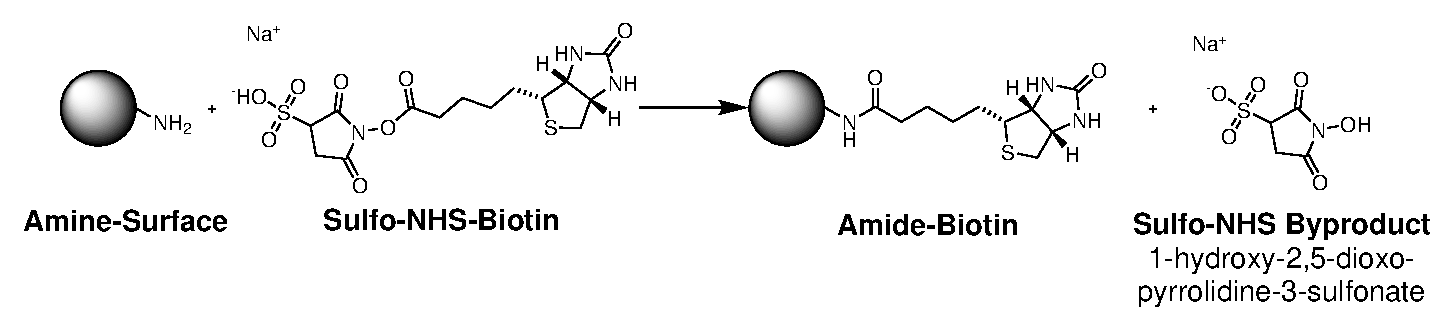
\includegraphics[width=\textwidth]{./Ressources/Chemistry/Sulfo-NHS.eps}
\caption{TestSvg}
\label{fig:Chem:NH2-NHS}
\end{figure}

\begin{figure}[hbtp]
\centering
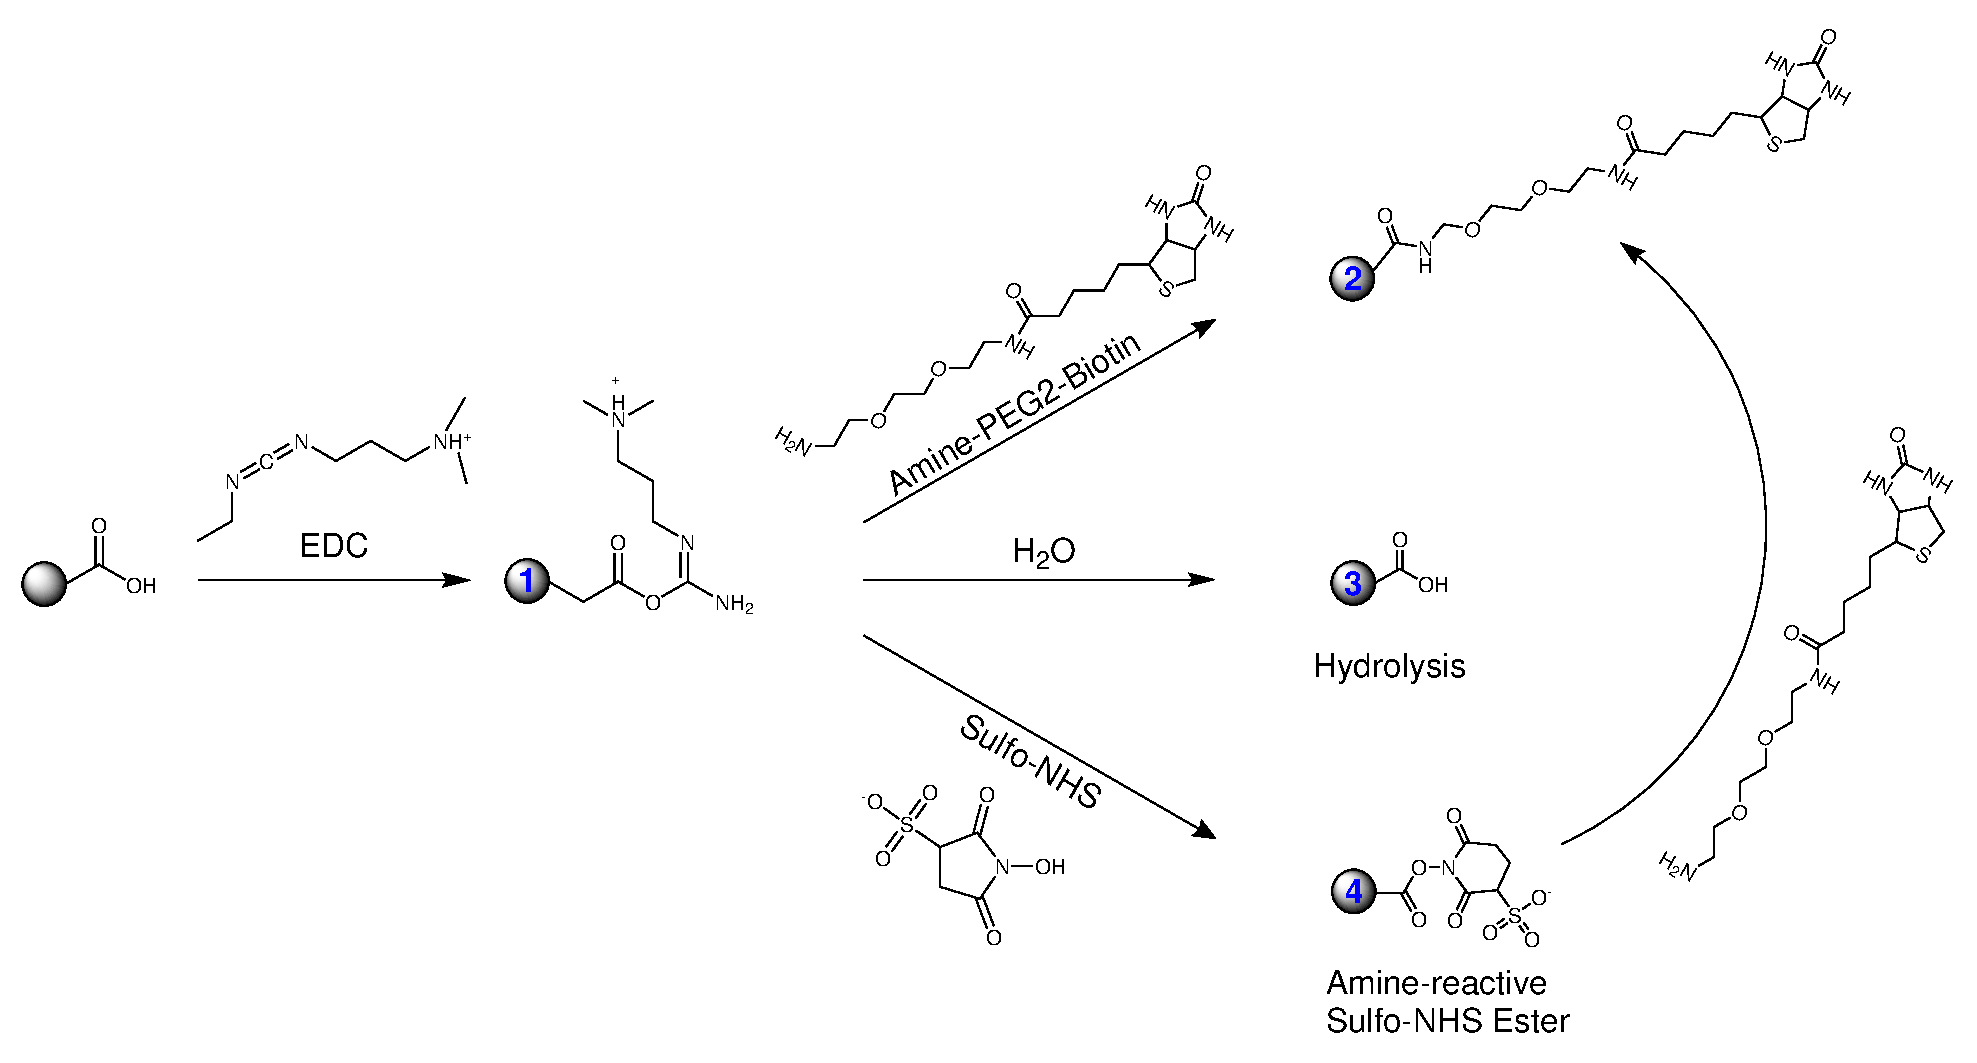
\includegraphics[width=\textwidth]{./Ressources/Chemistry/EDC-NHS.eps}
\caption{TestSvg}
\label{fig:Chem:COOH-EDC-NHS}
\end{figure}
\subsection{Microscopic Particle Surface Physics}

\subsection{The Biotin-Avidin-System}


\section{MRCyte}
Short intro over MRCyte
Foto of setup with arrows to necessary parts
Microscope
Stages
PEEK holder
Helmholtz coils
Kepco
MFLI
DAQ
\subsection{Focusing Structures}
test,test
Loss because of reduced velocity and magnetic drag
\subsection{GMR}
Different produced GMR stacks
Wheatstone Bridge setup
Magnet alignment
\subsection{Electrical Circuit}
Ground
PCB
Stacked PCBs with spacer
\subsection{Electronic Readout}
test,test
\subsubsection{Hysteresis Alignment}
test,test
\subsubsection{Single GMR}
test,test
\subsubsection{Dual GMR}
one MFLI supplies both at same freuqency. Aux Trigger tested, but no advantage.


